\documentclass{article}
\usepackage{graphicx} % Required for inserting images
\usepackage[spanish]{babel}
\usepackage{amssymb}
\usepackage{amsmath}
\usepackage{algorithm}
\usepackage{algpseudocode}
\usepackage{booktabs}
\usepackage{tabularx}
\usepackage{float}
\usepackage{booktabs}
\usepackage{xcolor}
\usepackage{makecell}
\usepackage{url}
\floatname{algorithm}{Algoritmo}


\title{Multiple Importance Sampling}
\author{santiolmedo99}
\date{July 2023}

\begin{document}

\maketitle

\section{Introducción}

En computación gráfica, los problemas de renderizado están llenos de problemas de integración.
Comúnmente, estás integrales son "difíciles", es decir, las funciones a integrar son discontinuas, multidimensionales o singulares y no tienen soluciones analíticas.
Es por ello que se recurre a métodos de resolución numéricos que permiten aproximar el valor de la integral con baja varianza.
Por la naturaleza de los problemas de renderizado, donde por ejemplo, se requiere renderizar cada pixel de una imagen en tiempo real, es necesario que los métodos de resolución sean eficientes en tiempo de ejecución y errores de estimación.
Los métodos comunes, como la integración trapezoidal o cuadratura de Gauss son efectivos para la resolución de problemas de baja dimensión pero no son escalables a los problemas que aparecen en computación gráfica.
La integración por Monte Carlo es particularmente atractivo porque su convergencia es independiente de la dimensionalidad del problema.

Otro atractivo del método de Monte Carlo es su facilidad de implementación. A priori, dado

$$ \int f(x) \,d(x)$$

solo se necesita la capacidad de evaluar $f(x)$ en un punto dado para poder estimar el valor de la integral.

Debido a los problemas de integración que aparecen en computación gráfica, es necesario recurrir a métodos de Monte Carlo que permitan reducir la varianza de la estimación.
En este trabajo se presenta la técnica de Multiple Importance Sampling (MIS) que permite combinar múltiples distribuciones de muestreo para reducir la varianza de la estimación.

El informe está organizado de la siguiente manera: en la sección 2 se presenta el método de Monte Carlo.
En la sección 3 se presenta la técnica de Multiple Importance Sampling y un estudio del estado del arte.
En la sección 4 se presentan los resultados de la implementación de MIS en un subconjunto de las heurísticas analizadas.
Esta comparación se basa en el tiempo de cálculo requerido para obtener una estimación precisa, el número de muestras requeridas y la variabilidad de las estimaciones (estimación de la varianza).


\section{Monte Carlo}

En general, los métodos numéricos que se fundamentan en la evaluación de \( n \) puntos dentro de un espacio de dimensión \( m \) para obtener una solución aproximada presentan un error que disminuye en el mejor de los casos en proporción a \( n^{-1/m} \).
Esta característica los hace extremadamente ineficientes en situaciones donde \( m \) es grande.

Por otro lado, los métodos de Monte Carlo generan estimaciones cuyo error absoluto es del orden de \( n^{-1/2} \), independientemente de la dimensión \( m \). Esta cualidad representa la ventaja principal del método y, en muchos casos, hace que sea la única opción viable.

Supongamos que deseo calcular un cierto valor $\phi$, y conozco una variable aleatoria $X$ con distribución $F_X$ tal que $\phi = \mathbb{E}(X)$. El método de Monte Carlo en su versión más simple consiste en:

\begin{algorithm}
\caption{Esquema básico de un Método Monte Carlo}
\begin{algorithmic}[1]

\State \textbf{sortear} valores para un conjunto $X^{(1)}, X^{(2)}, \dots, X^{(n)}$, de variables aleatorias i.i.d. (independientes e idénticamente distribuidas) a $X$.

\State Calcular $S_n = X^{(1)} + \dots + X^{(n)}$, la suma de los $n$ valores sorteados.

\State Calcular $\hat{X} = \frac{S_n}{n}$.

\State Calcular $\hat{V} = \left(\sum_{i=1}^{n} (X^{(i)})^2\right) / (n(n - 1)) - \hat{X}^2 / (n - 1)$.

\end{algorithmic}
\end{algorithm}

Se dice que $\hat{X}$ es un estimador de $\phi$ y $\hat{V}$ es un estimador de la varianza de $\hat{X}$.

Ahora, supongamos que se quiere evaluar el valor de la integral $I = \int_{a}^{b} f(x) \,dx$. Dado un conjunto de $n$ variables aleatorias $X_1, X_2, \dots, X_n$ independientes e idénticamente distribuidas con distribución $p(x)$, se puede decir que el valor esperado del estimador
$$F = \frac{b-a}{n} \sum_{i=1}^{n} f(X_i)$$
es igual a $I$. Esto se puede ver de la siguiente manera:
$$E[F] = E\left[\frac{b-a}{n} \sum_{i=1}^{n} f(X_i)\right] = \frac{b-a}{n} \sum_{i=1}^{n} E[f(X_i)] = \frac{b-a}{n} \sum_{i=1}^{n} \int_{a}^{b} f(x) p(x) \,dx = \int_{a}^{b} f(x) \,dx.$$
Dado que $X_i$ es muestreado de $[a,b]$, $p(x) = \frac{1}{b-a}$ para $x \in [a,b]$. Entonces, sustituyendo $p(x)$ por $\frac{1}{b-a}$, y haciendo $\frac{b-a}{n} * n = b-a$, se cancela con $\frac{1}{b-a}$, y se obtiene la última igualdad.

Esto se puede extender a
$$ F = \frac{1}{n} \sum_{i=1}^{n} \frac{f(X_i)}{p(X_i)}$$
es igual a I con la condición de que $p(x) > 0$. De manera parecida, se puede ver que el valor esperado del estimador:
$$E[F] = E\left[\frac{1}{n} \sum_{i=1}^{n} \frac{f(X_i)}{p(X_i)}\right] = \frac{1}{n} \sum_{i=1}^{n} \int_{a}^{b} \frac{f(x)}{p(x)} p(x) \,dx = \frac{1}{n} \sum_{i=1}^{n} \int_{a}^{b} f(x) \,dx = \int_{a}^{b} f(x) \,dx$$

Ahora, es importante mostrar el error de la estimación. Para esto, se puede usar el estimador del esquema básico de Monte Carlo para la varianza de $F$:

$$V[\frac{1}{n}\sum_{i=1}^{n} X_{(i)}] = \frac{1}{n^{2}} \sum_{i=1}^{n} V[X_{(i)}]$$

dado que las variables aleatorias $X_{i}$ son independientes. Teniendo en cuenta que $X_{i}$ tienen la misma distribución y por lo tanto la misma varianza, se puede escribir:

$$V[F] = \frac{1}{n^{2}} \sum_{i=1}^{n} V[X_{(i)}] = \frac{1}{n^{2}} * n * \sigma^{2} = \frac{\sigma^{2}}{n}$$.

Por lo tanto, el error de la estimación es $\frac{\sigma^{2}}{n}$, que es del orden de $n^{-1/2}$.

El estimador que se obtinene es insesgado, es decir, $E[F] = I$. Cuando el estimador es sesgado, la diferencia:

$$\beta = E[F] - I$$

es el sesgo.

\section{Multiple Importance Sampling}

En esta sección se va a presentar la técnica de Multiple Importance Sampling (MIS) y un estudio del estado del arte.

\subsection{Motivación}

Tenemos una integral que puede ser de de la forma
$$ \int f_{1}(x) * f_{2}(x) * f_{3}(x) * ... * f_{k}(x) \,d(x)$$

y $ p_{1}, p_{2}, p_{3}, ..., p_{k}$ proporcionales a $f_{1}, f_{2}, f_{3}, ..., f_{k}$.
La idea es usar las distintas distribuciones de muestreo y combinarlas para encontrar una estimación de la integral con menor varianza y en poco tiempo de cómputo.

El problema también es que la inherencia de la computación gráfica hace que las funciones a integrar dependan de varios parámetros del modelo de la escena.
Esto hace que sea difícil encontrar una distribución de muestreo que sea buena para todos los parámetros.
Por lo tanto, se puede usar MIS para combinar varias distribuciones de muestreo y obtener una estimación con menor varianza para todo el espacio de parámetros.

En las próximas subsecciones se van a presentar las técninas para combinas las distribuciones de muestreo.
No se explica cómo conseguir las distribuciones de muestreo, sino que se asume que se tienen las distribuciones de muestreo y se trabaja sobre conseguir combinaciones que permitan construir un estimador con menor varianza.

\subsection{Veach}

Veach propone en su tesis técnicas para combinas las distribuciones y obtener un estimador con varianza baja y demostrablemente bueno.
En su tesis presenta el modelo multi-sample y distintas heurísticas para combinar las distribuciones de muestreo.
A su vez, presenta el modelo one-sample que consiste en elegir en cada corrida una distribución de muestreo y usarla para estimar la integral.

\subsubsection{Modelo multi-sample}

Queremos estimar:

$$ \int f_(x) \,d\mu(x)$$

donde el dominio de integración es $\Omega$ y $\mu$ es dado. Tenemos $n$ distribuciones de muestreo $p_{1}, p_{2}, ..., p_{n}$, en el dominio $\Omega$.
Tenemos las siguientes operaciones:
\begin{itemize}
    \item dado $x \in \Omega$, podemos evaluar $f(x)$ y $p_{i}(x)$
    \item la posibilidad de generar una muestra X con distribución $p_{i}$
\end{itemize}

Notación:
\begin{itemize}
    \item $n_{i}$: número de muestras generadas con $p_{i}$. Este numéro es conocido a priori.
    \item $N = \sum_{i=1}^{n} n_{i}$: número total de muestras
    \item Para $j \in \{1, 2, ..., N\}$, $X_{i,j}$ es la $j$-ésima muestra generada con $p_{i}$
\end{itemize}

\subsubsection{Estimador multi-sample}

Objetivo: encontrar un estimador insesgado combinando las muestras generadas con las distintas distribuciones de muestreo.
Para esto, consideramos estimadores que le dan pesos diferentes a cada muestra.
El estimador multi-sample es de la forma:

$$F = \sum_{i=1}^{n} \frac{1}{n_{i}} \sum_{j=1}^{n_{i}} w_{i}(X_{i,j}) \frac{f(X_{i,j})}{p_{i}(X_{i,j})}$$

donde se tiene que cumplir que:

\begin{itemize}
    \item $\sum_{i=1}^{n} w_{i}(x) = 1$ si $f(x) \neq 0$
    \item $w_{i}(x) = 0$ si $p_{i}(x) = 0$
\end{itemize}

Esto implica que en cada punto donde f(x) es distinto de 0, al menos una de $p_{i}(x)$ es positivo.

Lema de que el estimador es insesgado:

$$E[F] = \int f_(x) \,d\mu(x)$$

Podemos demostrar que:
\begin{align*}
E[F] &= E\left[\sum_{i=1}^n \frac{1}{n_i} \sum_{j=1}^{n_i} w_i(X_{i,j}) \frac{f(X_{i,j})}{p_i(X_{i,j})}\right] \\
&= \sum_{i=1}^n \frac{1}{n_i} E\left[\sum_{j=1}^{n_i} w_i(X_{i,j}) \frac{f(X_{i,j})}{p_i(X_{i,j})}\right] \\
&= \sum_{i=1}^n \frac{1}{n_i} \sum_{j=1}^{n_i} \int_{\Omega} w_i(x) \frac{f(x)}{p_i(x)} p_i(x) d\mu(x) \\
&= \int_{\Omega} \left(\sum_{i=1}^n w_i(x)\right) f(x) d\mu(x) \\
&= \int_{\Omega} f(x) d\mu(x),
\end{align*}
dado que por la condición \( (W1) \), \( \sum_{i=1}^n w_i(x) = 1 \) siempre que \( f(x) \neq 0 \).

Por lo tanto, el estimador \( F \) es imparcial. La última igualdad se debe a que \( \sum_{i=1}^n w_i(x) = 1 \) cuando \( f(x) \neq 0 \).

\subsubsection{Balance Heurística}

$$ w_{i}(x) = \frac{n_{i} * p_{i}(x)}{\sum_{k} n_{k} * p_{k}(x)}$$

\textbf{Teorema 9.2} Dado $f$, $n_{i}$ y $p_{i}$ para $i \in \{1, 2, ..., n\}$. Sea F cualquier estimador insesgado de la forma del multi-sample estimator y $\hat{F}$ el estimador balance heuristic. Entonces:

$$V[\hat{F}] - V[F] \leq ( \frac{1}{min_{i} n_{i}} - \frac{1}{\sum_{i} n_{i}} ) * \mu^{2}$$

donde $\mu = E[F] = E[\hat{F}]$.

% \textbf{Demostración}:

% Sean:

% $$ F_{i}{j} = \frac{w_{i}(X_{i,j}) f(X_{i,j})}{p_{i}(X_{i,j})}$$

% y

% $$ \mu_{i} = E[F_{i}{j}] =  \int_{\Omega} w_{i}(x) f(x) d\mu(x)$$.

% Entonces:

% \begin{align*}
%   V[F] &= V\left[\sum_{i=1}^n \frac{1}{n_i} \sum_{j=1}^{n_i} F_{i,j}\right] \\
%   &= \sum_{i=1}^n \frac{1}{n_i^2} \sum_{j=1}^{n_i} V[F_{i,j}] \\
%   &= \left(\sum_{i=1}^n \frac{1}{n_i^2} \sum_{j=1}^{n_i} E[F_{i,j}^2]\right) - \left(\sum_{i=1}^n \frac{1}{n_i^2} \sum_{j=1}^{n_i} E[F_{i,j}]^2\right) \\
%   &= \left(\sum_{i=1}^n \frac{1}{n_i^2} \sum_{j=1}^{n_i} \int_{\Omega} \frac{w_i(x)^2 f(x)^2}{p_i(x)^2} p_{i}(x) d\mu(x)\right) - \left(\sum_{i=1}^n \frac{1}{n_i^2} n_i  \mu_i^2\right) \\
%   &= \int_{\Omega} \left(\sum_{i=1}^n \frac{w_i(x)^2 f(x)^2}{n_i p_i(x)} d\mu(x)\right) - \left(\sum_{i=1}^n \frac{\mu_i^2}{n_i}\right).
% \end{align*}

% ... seguir viendo y entendiendo la demostración.

\subsubsection{Otras Heurísticas}

Dentro de los límites presentados en el Teorema 9.2, Veach presenta más heurísticas que son demostrablemente mejores que balance heuristic en circinstancias particulares.
Estas heurísticas son insesgadas al igual que balance heuristic.

Se considera la situación donde una de las distribuciones de muestreo es un match perfecto para la función a integrar. En este caso, es deseable que la heurística le de un peso de 1 a esta distribución de muestreo y 0 a las demás. (hacer referencia a la imagen)
La idea entonces es ir sampleando con las distintas distribuciones de muestreo y darle un peso de 1 en todo el dominio a la distribución de muestreo cercana a $f$ y 0 a las demás.
Sería como tomar muestras solo de la distribución de muestreo cercana a $f$ pero de igual manera tomando muestras de todas porque no se sabe de antemano cuál es la distribución de muestreo cercana a $f$.

Para encontrar la heurística se toma como ejemplo la función donde $p1$ es un match perfecto para $f$ y $p2$ es una constante.
Se quiere encontrar una heurística que le de un peso de 1 a $p1$ y 0 a $p2$.

\section{Experimentación práctica}

Dentro de esta sección se presenta la implementación del MIS en un conjunto de pruebas que va a permitir analizar el comportamiento de MIS en distintos escenarios.

\subsection{Prueba 1 - Análisis de un caso simple}

La primera función se utilizó para familiarizarse con el algoritmo y verificar que el código implementado funcionaba correctamente.
Se corroboró la correctitud del MIS implementado usando distintas heurísticas y se utilizó el código como base para las pruebas siguientes.

\subsubsection{Función}
La función que examinamos se define para un conjunto de valores \( x \) y rangos específicos. Para cada rango \( [a_{i}, b_{i}] \), la función se expresa como:
$$
f(x) = \sum_{i} \max\left(0, -\frac{4}{(b_{i} - a_{i})^2} (x - a_{i})(x - b_{i})\right)
$$
Aquí, la suma se lleva a cabo sobre los diferentes rangos considerados.

\subsubsection{Distribuciones de Muestreo}

Para tomar las muestras, se consideraron 3 distribuciones de muestreo \( p_{i}(x) \) para cada rango \( [a_{i}, b_{i}] \).
La distribución de muestreo \( p_{i}(x) \) se definió como una distribución normal con media \( \mu_{i} \) y desviación estándar \( \sigma_{i} \).

Luego, la PDF utilizada corresponde a la de una distribución normal, caracterizada por una media \( \mu \) y una desviación estándar \( \sigma \). La fórmula es la siguiente:
$$
p(x) = \frac{1}{\sigma \sqrt{2\pi}} \exp\left(-\frac{(x - \mu)^2}{2\sigma^2}\right)
$$


\subsubsection{Ejemplo}

Para poder visualizar la función se considera el siguiente ejemplo donde:

\begin{itemize}
    \item \textbf{\( \mu_{i} \)}: [5, 10, 15]
    \item \textbf{\( \sigma_{i} \)}: [1.0, 0.5, 0.75]
    \item \textbf{\( a_{i} \)}: [3.0, 9.0, 13.5]
    \item \textbf{\( b_{i} \)}: [7.0, 11.0, 16.5]
\end{itemize}

En la figura \ref{fig:mis1} se puede ver la función \( f(x) \) y las distribuciones de muestreo \( p_{i}(x) \) para cada rango \( [a_{i}, b_{i}] \).
A su vez, se hizo una corrida con balance heuristic y se puede ver en rojo los puntos muestreados.

\begin{figure}[H]
\includegraphics[width=1\textwidth]{Figure_1_mis.png}
\caption{Función \( f(x) \) y distribuciones de muestreo \( p_{i}(x) \) para cada rango \( [a_{i}, b_{i}] \).}
\label{fig:mis1}
\end{figure}

\subsubsection{Pruebas realizadas}

Sobre este caso de prueba se generó un análisis de las distintas heurísticas implementadas.
Para el análisis se hizo lo siguiente:
\begin{itemize}
    \item Se hicieron 10 tests diferentes. Para cada test se generaron valores aleatiorios para \( \mu_{i} \), \( \sigma_{i} \), \( a_{i} \) y \( b_{i} \).
          Por simplicidad, para el primer rango de  \( \mu_{i} \) se fijaron los valores entre 2 y 7.
          Para el segundo rango de \( \mu_{i} \) se fijaron los valores entre 7 y 12.
          Para el tercer rango de \( \mu_{i} \) se fijaron los valores entre 12 y 18.
          Las desviaciones estándar \( \sigma_{i} \) se fijaron entre 0.01 y 1.
          Los rangos \( [a_{i}, b_{i}] \) se calcularon como \( [ \mu_{i} - 2 * \sigma_{i}, \mu_{i} + 2 * \sigma_{i} ] \).
    \item Para cada test se corrió MIS con las siguientes heurísticas: balance, power, maximum, cutoff y sbert.
    \item Para cada heurística se corrió MIS con 10, 25, 50, 100 y 150 muestras.
    \item Para cada heurística y cantidad de muestras se corrió MIS 100 veces y se calculó el promedio de las estimaciones,
          el promedio de la varianza de las estimaciones y el promedio de las desviaciones estándar de las estimaciones.
          A su vez, se calculó el promedio de los errores comparados con una estimación hecha con quad y el promedio del tiempo de cómputo.
\end{itemize}

Una, vez hecho esto, debido a la extensión de los resultados, se decidió hacer el siguiente análisis de la varianza de las estimaciones, las desviaciones estándar de las estimaciones, el error de las estimaciones y el promedio del error de las desviaciones en comparación con el método de cuadratura.
Esto último se decidió ya que no se cuenta con un cálculo exacto de la integral y se decidió usar el método de cuadratura como referencia.
Este análisis se hizo para:

\begin{itemize}
    \item Cada heurística y cantidad de muestras combinadas.
    \item Cada heurística dentro de cada test.
    \item Cada heurística.
\end{itemize}

\subsubsection{Resultados}

\begin{table}[H]
\centering
\label{table:heuristic_sample_analysis}
\small
\setlength{\tabcolsep}{3pt}
\renewcommand{\arraystretch}{1.2}
\begin{tabular}{|l|r|r|r|r|r|}
\hline
\textbf{\makecell{Heurística / \\ \# de muestras}} & \textbf{10} & \textbf{25} & \textbf{50} & \textbf{100} & \textbf{150} \\ \hline
\multicolumn{6}{|c|}{\textbf{Promedio de Var}} \\ \hline
Balance & 0.4441 & 0.1579 & 0.0735 & 0.0376 & 0.0247 \\ \hline
Power & 0.4505 & 0.1615 & 0.0749 & 0.0384 & 0.0253 \\ \hline
Maximum & 0.4766 & 0.1719 & 0.0797 & 0.0408 & 0.0269 \\ \hline
Cutoff & 0.4575 & 0.1642 & 0.0760 & 0.0389 & 0.0257 \\ \hline
Sbert & 0.4423 & 0.1584 & 0.0734 & 0.0374 & 0.0247 \\ \hline
\multicolumn{6}{|c|}{\textbf{Promedio de Err}} \\ \hline
Balance & 0.0122 & 0.0062 & 0.0036 & 0.0028 & 0.0019 \\ \hline
Power & 0.0078 & 0.0062 & 0.0051 & 0.0039 & 0.0024 \\ \hline
Maximum & 0.0135 & 0.0066 & 0.0041 & 0.0015 & 0.0015 \\ \hline
Cutoff & 0.0089 & 0.0068 & 0.0058 & 0.0045 & 0.0032 \\ \hline
Sbert & 0.0148 & 0.0059 & 0.0031 & 0.0042 & 0.0033 \\ \hline
\multicolumn{6}{|c|}{\textbf{Promedio de DE}} \\ \hline
Balance & 0.6009 & 0.3674 & 0.2533 & 0.1818 & 0.1477 \\ \hline
Power & 0.6059 & 0.3727 & 0.2563 & 0.1843 & 0.1496 \\ \hline
Maximum & 0.6238 & 0.3848 & 0.2646 & 0.1900 & 0.1545 \\ \hline
Cutoff & 0.6112 & 0.3762 & 0.2583 & 0.1856 & 0.1510 \\ \hline
Sbert & 0.6003 & 0.3685 & 0.2533 & 0.1815 & 0.1475 \\ \hline
\end{tabular}
\caption{Análisis de los resultados por heurística y cantidad de muestras}
\label{table:heuristic_analysis}
\end{table}


\begin{table}[H]
\centering
\label{table:heuristic_test_analysis}
\resizebox{\textwidth}{!}{%
\begin{tabular}{|c|c|c|c|}
\hline
\textbf{Heurística/Test} & \textbf{Promedio de Var} & \textbf{Promedio de Err} & \textbf{Promedio de DE} \\ \hline
\multicolumn{4}{|c|}{\textbf{Test 1}} \\ \hline
Balance & 0.1039 & 0.0067 & 0.2665 \\ \hline
Power & 0.1015 & 0.0103 & 0.2645 \\ \hline
Maximum & 0.1023 & 0.0024 & 0.2657 \\ \hline
Cutoff & 0.1026 & 0.0091 & 0.2646 \\ \hline
Sbert & 0.1035 & 0.0050 & 0.2662 \\ \hline
\multicolumn{4}{|c|}{\textbf{Test 2}} \\ \hline
Balance & 0.1625 & 0.0055 & 0.3500 \\ \hline
Power & 0.1640 & 0.0081 & 0.3512 \\ \hline
Maximum & 0.1641 & 0.0065 & 0.3518 \\ \hline
Cutoff & 0.1628 & 0.0075 & 0.3507 \\ \hline
Sbert & 0.1630 & 0.0060 & 0.3501 \\ \hline
\multicolumn{4}{|c|}{\textbf{Test 3}} \\ \hline
Balance & 0.0907 & 0.0047 & 0.2497 \\ \hline
Power & 0.0912 & 0.0040 & 0.2503 \\ \hline
Maximum & 0.0890 & 0.0082 & 0.2480 \\ \hline
Cutoff & 0.0936 & 0.0076 & 0.2531 \\ \hline
Sbert & 0.0950 & 0.0139 & 0.2543 \\ \hline
\multicolumn{4}{|c|}{\textbf{Test 4}} \\ \hline
Balance & 0.3690 & 0.0088 & 0.5303 \\ \hline
Power & 0.3670 & 0.0045 & 0.5295 \\ \hline
Maximum & 0.3659 & 0.0054 & 0.5288 \\ \hline
Cutoff & 0.3675 & 0.0038 & 0.5296 \\ \hline
Sbert & 0.3644 & 0.0032 & 0.5278 \\ \hline
\multicolumn{4}{|c|}{\textbf{Test 5}} \\ \hline
Balance & 0.0929 & 0.0062 & 0.2582 \\ \hline
Power & 0.1225 & 0.0084 & 0.2969 \\ \hline
Maximum & 0.2178 & 0.0118 & 0.3975 \\ \hline
Cutoff & 0.1440 & 0.0082 & 0.3215 \\ \hline
Sbert & 0.0920 & 0.0083 & 0.2575 \\ \hline
\end{tabular}%
}
\caption{Análisis de los resultados por heurística en los tests 1-5}
\end{table}

\begin{table}[H]
\centering
\label{table:heuristic_test_analysis}
\resizebox{\textwidth}{!}{%
\begin{tabular}{|c|c|c|c|}
\hline
\textbf{Heurística/Test} & \textbf{Promedio de Var} & \textbf{Promedio de Err} & \textbf{Promedio de DE} \\ \hline
\multicolumn{4}{|c|}{\textbf{Test 6}} \\ \hline
Balance & 0.2760 & 0.0057 & 0.4588 \\ \hline
Power & 0.2763 & 0.0032 & 0.4590 \\ \hline
Maximum & 0.2750 & 0.0045 & 0.4584 \\ \hline
Cutoff & 0.2748 & 0.0062 & 0.4581 \\ \hline
Sbert & 0.2740 & 0.0086 & 0.4578 \\ \hline
\multicolumn{4}{|c|}{\textbf{Test 7}} \\ \hline
Balance & 0.0882 & 0.0029 & 0.2594 \\ \hline
Power & 0.0878 & 0.0029 & 0.2590 \\ \hline
Maximum & 0.0874 & 0.0023 & 0.2585 \\ \hline
Cutoff & 0.0877 & 0.0037 & 0.2589 \\ \hline
Sbert & 0.0879 & 0.0029 & 0.2590 \\ \hline
\multicolumn{4}{|c|}{\textbf{Test 8}} \\ \hline
Balance & 0.0354 & 0.0023 & 0.1630 \\ \hline
Power & 0.0352 & 0.0015 & 0.1628 \\ \hline
Maximum & 0.0353 & 0.0030 & 0.1628 \\ \hline
Cutoff & 0.0347 & 0.0047 & 0.1620 \\ \hline
Sbert & 0.0357 & 0.0020 & 0.1636 \\ \hline
\multicolumn{4}{|c|}{\textbf{Test 9}} \\ \hline
Balance & 0.2219 & 0.0026 & 0.4122 \\ \hline
Power & 0.2221 & 0.0049 & 0.4124 \\ \hline
Maximum & 0.2220 & 0.0052 & 0.4124 \\ \hline
Cutoff & 0.2224 & 0.0025 & 0.4126 \\ \hline
Sbert & 0.2230 & 0.0098 & 0.4128 \\ \hline
\multicolumn{4}{|c|}{\textbf{Test 10}} \\ \hline
Balance & 0.0351 & 0.0081 & 0.1543 \\ \hline
Power & 0.0337 & 0.0031 & 0.1521 \\ \hline
Maximum & 0.0332 & 0.0054 & 0.1515 \\ \hline
Cutoff & 0.0348 & 0.0049 & 0.1538 \\ \hline
Sbert & 0.0340 & 0.0029 & 0.1529 \\ \hline
\end{tabular}%
}
\caption{Análisis de los resultados por heurística en los tests 6-10}
\end{table}

\begin{table}[H]
\centering
\label{table:heuristic_analysis}
\resizebox{\textwidth}{!}{%
\begin{tabular}{|c|c|c|c|}
\hline
\textbf{Heurística} & \textbf{Promedio de Var} & \textbf{Promedio de Err} & \textbf{Promedio de DE} \\ \hline
Balance & 0.1476 & 0.0054 & 0.3102 \\ \hline
Power & 0.1501 & 0.0051 & 0.3138 \\ \hline
Maximum & 0.1592 & 0.0055 & 0.3235 \\ \hline
Cutoff & 0.1525 & 0.0058 & 0.3165 \\ \hline
Sbert & 0.1473 & 0.0063 & 0.3102 \\ \hline
\end{tabular}%
}
\caption{Análisis de los resultados por heurística}
\end{table}


\paragraph{Diferencias entre Heurísticas}
Varianza de las Estimaciones: Las heurísticas 'Balance' y 'Sbert' muestran consistentemente las varianzas más bajas a través de todos los tamaños de muestra, lo que indica una mayor precisión en sus estimaciones.
Por otro lado, 'Maximum' presenta la varianza más alta, especialmente con tamaños de muestra más pequeños, lo que sugiere una menor fiabilidad en comparación con otras heurísticas.

Error de las Estimaciones: 'Balance' y 'Sbert' muestran los números más bajos para los errores, lo que indica una mayor precisión en sus resultados.
Las heurísticas 'Maximum' y 'Cutoff' presentan errores más significativos.

Desviaciones Estándar de las Estimaciones: Las heurísticas 'Balance', 'Power', y 'Sbert' mantienen desviaciones estándar más bajas, lo que sugiere estimaciones más consistentes.
'Maximum' presenta la mayor desviación estándar, reafirmando su menor consistencia en las estimaciones.

\paragraph{Competitividad del MIS en Función del Tamaño de Muestra}
Se observa que a medida que el tamaño de la muestra aumenta, todas las heurísticas mejoran en términos de varianza, error, y desviación estándar de las estimaciones. Esto es un indicativo de que el MIS se vuelve más competitivo y confiable con un mayor número de muestras.
Específicamente, con tamaños de muestra de 50 en adelante, se empieza a notar una mejora significativa en la precisión y consistencia de las estimaciones para todas las heurísticas.
Las heurísticas 'Balance' y 'Sbert' demuestran ser competitivas incluso con tamaños de muestra más pequeños (25 muestras), mientras que otras heurísticas como 'Maximum' y 'Cutoff' requieren tamaños de muestra mayores para alcanzar niveles similares de precisión y confiabilidad.

En resumen, las heurísticas 'Balance' y 'Sbert' muestran un rendimiento superior en términos de varianza, error y consistencia de las estimaciones a través de todos los tamaños de muestra. El MIS se vuelve notablemente más competitivo y preciso con tamaños de muestra de 50 o más, aunque algunas heurísticas como 'Balance' y 'Sbert' ya muestran resultados prometedores con tamaños de muestra de 25. En contraste, heurísticas como 'Maximum' y 'Cutoff' requieren tamaños de muestra más grandes para ofrecer un nivel de precisión y consistencia comparable.

\subsection{Prueba 2 - Análisis Multidimensional}

En esta sección, nos centramos en el análisis de una función multidimensional basada en la función hiperbólica \textit{sech}, extendida a múltiples dimensiones. La función \textit{sech}, definida como \( \text{sech}(x) = \frac{2}{e^x + e^{-x}} = \frac{1}{\cosh(x)} \), es conocida por su similitud con la distribución gaussiana en una dimensión, especialmente cerca del origen.

La función objetivo, \( h(\mathbf{x}) \), donde \( \mathbf{x} \) es un vector \( n \)-dimensional, es expresada como una suma de \( m \) funciones \( f_i(\mathbf{x}) \):
\[ h(\mathbf{x}) = \sum_{i=1}^{m} f_i(\mathbf{x}) \]
donde cada \( f_i(\mathbf{x}) \) es definida por:
\[ f_i(\mathbf{x}_1, \mathbf{x}_2, \ldots, \mathbf{x}_n) = \prod_{j=1}^{n} \text{sech}(a_{ij} (x_j - b_{ij})) \]

Aquí, \( a_{ij} \) y \( b_{ij} \) son constantes positivas que determinan la anchura y la posición de la función \( f_i \) en la dimensión \( j \), respectivamente.

Para calcular el volumen (integral) de esta función sobre el espacio \( n \)-dimensional, consideramos la integral de cada componente \textit{sech}, que se simplifica a \( \frac{\pi}{a_i} \) para cada dimensión. Por lo tanto, el volumen total se obtiene como:
\[ V = \sum_{i=1}^{m} \prod_{i=1}^{n} \frac{\pi}{a_i} = \sum_{i=1}^{m} \frac{\pi^n}{\prod_{i=1}^{n} a_i} \]

Para la aproximación gaussiana de la función \textit{sech} en múltiples dimensiones, consideramos gaussianas estándar con medias centradas y desviaciones estándar ajustadas.
La correspondencia entre las \"anchuras\" de las funciones \textit{sech} y las desviaciones estándar de las gaussianas se establece mediante un mapeo aproximado, asegurando que ambas funciones tengan anchuras comparables en el punto donde caen a la mitad de su valor máximo.

\color{red}
aca se podria explicar mas lo que se hizo con el sigma
\color{black}

El objetivo principal de este análisis es aplicar el MIS para estimar la integral de una función compleja, que es una suma de funciones \textit{sech} multidimensionales, a través de varias distribuciones propuestas.
Esta función nos va a permitir analizar el MIS en varias dimensiones y comparar las diferentes heurísticas implementadas.

En las siguientes subsecciones, detallaremos la implementación y los resultados de aplicar MIS a esta función multidimensional, examinando la eficacia de diferentes estrategias de muestreo y distribuciones propuestas.

\subsubsection{Ejemplo}

Para poder visualizar la función se considera el siguiente ejemplo donde:

\begin{itemize}
    \item \textbf{\( a_{ij} \)}: [[2, 2], [2, 2], [2, 2]]
    \item \textbf{\( b_{ij} \)}: [[39, -7], [45, -37], [-36, -3]]
\end{itemize}

En la figura \ref{fig:mis2} se puede ver la función \( f(x) \) y las distribuciones de muestreo \( p_{i}(x) \) para cada rango \( [a_{i}, b_{i}] \).
A su vez, se hizo una corrida con balance heuristic y ver en rojo, verde y azul los puntos muestreados.

\begin{figure}[H]
\includegraphics[width=1\textwidth]{Figure_2_mis.png}
\caption{Función \( f(x) \) y distribuciones de muestreo \( p_{i}(x) \) para cada rango \( [a_{i}, b_{i}] \).}
\label{fig:mis2}
\end{figure}

\subsubsection{Pruebas realizadas}

Sobre este caso de prueba se generó un análisis de las distintas heurísticas implementadas.
Para el análisis se hizo lo siguiente:
\begin{itemize}
    \item Se hicieron 10 tests diferentes. Para cada test se generaron valores aleatiorios para \( a_{ij} \), \( b_{ij} \), \( m \) y \( n \).
          En cada test se generó un número aleatiorio entre 2 y 10 para \( m \) y \( n \) se fijó en el número del test.
          Es decir, para el primer test \( n = 1 \), para el segundo test \( n = 2 \), etc. La dimensión entonces es el número del test más 1.
          Para cada test se generaron valores aleatiorios para \( a_{ij} \) entre 1.8 y 2.
          Para cada test se generaron valores aleatiorios para \( b_{ij} \) entre -100 y 100.
    \item Para cada test se corrió MIS con las siguientes heurísticas: balance, power, maximum, cutoff y sbert.
    \item Para cada heurística se corrió MIS con 50, 100, 500, 1000 y 5000 muestras.
    \item Para cada heurística y cantidad de muestras se corrió MIS 100 veces y se calculó el promedio de las estimaciones,
          el promedio de la varianza de las estimaciones y el promedio de las desviaciones estándar de las estimaciones.
          A su vez, se calculó el promedio de los errores comparados el valor exacto de la integral y el promedio del tiempo de cómputo.
\end{itemize}

De la misma manera que para la prueba pasada, se hizo un resumen de los resultados debido a la extensión de los mismos.
Se hizo el siguiente análisis de la varianza de las estimaciones, las desviaciones estándar de las estimaciones, el error de las estimaciones.

El análisis se hizo para los mismos casos que en la prueba anterior.

\subsubsection{Resultados}

\begin{table}[H]
\centering
\label{table:heuristic_sample_analysis}
\small
\setlength{\tabcolsep}{3pt}
\renewcommand{\arraystretch}{1.2}
\begin{tabular}{|l|r|r|r|r|r|}
\hline
\textbf{\makecell{Heurística / \\ \# de muestras}} & \textbf{50} & \textbf{100} & \textbf{500} & \textbf{1000} & \textbf{5000} \\ \hline
\multicolumn{6}{|c|}{\textbf{Promedio de Var}} \\ \hline
Balance & 28542.80 & 11755.25 & 32890.92 & 2082.61 & 1470.44 \\ \hline
Power & 16022.84 & 136709.92 & 3707.40 & 75721.90 & 2557.03 \\ \hline
Maximum & 16750.33 & 16552.90 & 111964.69 & 3072.33 & 7038.19 \\ \hline
Cutoff & 23826.31 & 236449.12 & 74333.52 & 5878.86 & 1416.80 \\ \hline
Sbert & 6603.14 & 59408.55 & 17053.03 & 1951.91 & 7476.45 \\ \hline
\multicolumn{6}{|c|}{\textbf{Promedio de Err}} \\ \hline
Balance & 3.63 & 8.93 & -1.65 & 6.80 & 6.29 \\ \hline
Power & 10.67 & -6.78 & 5.86 & -1.69 & 2.84 \\ \hline
Maximum & 8.21 & 5.28 & -6.80 & 5.43 & 1.24 \\ \hline
Cutoff & 8.08 & -12.71 & 0.51 & 2.23 & 4.12 \\ \hline
Sbert & 13.10 & -0.75 & 0.52 & 7.51 & 0.67 \\ \hline
\multicolumn{6}{|c|}{\textbf{Promedio de DE}} \\ \hline
Balance & 40.21 & 31.19 & 29.39 & 17.13 & 10.70 \\ \hline
Power & 36.94 & 46.45 & 21.71 & 26.32 & 13.61 \\ \hline
Maximum & 36.01 & 34.19 & 34.76 & 18.94 & 15.45 \\ \hline
Cutoff & 37.73 & 46.92 & 28.03 & 21.41 & 12.85 \\ \hline
Sbert & 32.84 & 39.51 & 27.41 & 16.83 & 15.55 \\ \hline
\end{tabular}%
}
\caption{Análisis de los resultados por heurística y cantidad de muestras}
\end{table}

\begin{table}[H]
\centering
\label{table:heuristic_test_analysis}
\resizebox{\textwidth}{!}{%
\begin{tabular}{|c|c|c|c|}
\hline
\textbf{Heurística/Test} & \textbf{Promedio de Var} & \textbf{Promedio de Err} & \textbf{Promedio de DE} \\ \hline
\multicolumn{4}{|c|}{\textbf{Test 1 (2 dimensiones)}} \\ \hline
Balance & 0.04 & 0.03 & 0.12 \\ \hline
Power & 0.12 & 0.00 & 0.15 \\ \hline
Maximum & 30.53 & -0.24 & 0.40 \\ \hline
Cutoff & 0.07 & 0.01 & 0.14 \\ \hline
Sbert & 0.06 & 0.02 & 0.13 \\ \hline
\multicolumn{4}{|c|}{\textbf{Test 2 (3 dimensiones)}} \\ \hline
Balance & 1.86 & 0.11 & 0.52 \\ \hline
Power & 0.76 & 0.11 & 0.50 \\ \hline
Maximum & 8.76 & 0.00 & 0.62 \\ \hline
Cutoff & 1.07 & 0.12 & 0.51 \\ \hline
Sbert & 2.64 & -0.02 & 0.64 \\ \hline
\multicolumn{4}{|c|}{\textbf{Test 3 (4 dimensiones)}} \\ \hline
Balance & 29.51 & 0.49 & 2.21 \\ \hline
Power & 105.99 & -0.14 & 2.86 \\ \hline
Maximum & 18.16 & 0.70 & 2.06 \\ \hline
Cutoff & 23.96 & 0.28 & 2.43 \\ \hline
Sbert & 278.20 & 0.10 & 2.65 \\ \hline
\multicolumn{4}{|c|}{\textbf{Test 4 (5 dimensiones)}} \\ \hline
Balance & 18.61 & 0.27 & 1.62 \\ \hline
Power & 85.91 & -0.21 & 2.14 \\ \hline
Maximum & 40.65 & -0.12 & 1.95 \\ \hline
Cutoff & 9.87 & 0.46 & 1.47 \\ \hline
Sbert & 9.34 & 0.37 & 1.54 \\ \hline
\multicolumn{4}{|c|}{\textbf{Test 5 (6 dimensiones)}} \\ \hline
Balance & 481.61 & 2.76 & 11.17 \\ \hline
Power & 943.69 & 2.36 & 11.74 \\ \hline
Maximum & 1771.43 & 0.04 & 14.19 \\ \hline
Cutoff & 863.24 & 0.92 & 13.37 \\ \hline
Sbert & 724.53 & 1.85 & 12.35 \\ \hline
\end{tabular}%
}
\caption{Análisis de los resultados por heurística en los tests 1-5}
\end{table}

\begin{table}[H]
\centering
\label{table:heuristic_test_analysis}
\resizebox{\textwidth}{!}{%
\begin{tabular}{|c|c|c|c|}
\hline
\textbf{Heurística/Test} & \textbf{Promedio de Var} & \textbf{Promedio de Err} & \textbf{Promedio de DE} \\ \hline
\multicolumn{4}{|c|}{\textbf{Test 6 (7 dimensiones)}} \\ \hline
Balance & 1306.95 & 2.46 & 15.34 \\ \hline
Power & 963.76 & 3.33 & 14.93 \\ \hline
Maximum & 9279.05 & -0.52 & 18.93 \\ \hline
Cutoff & 1088.97 & 3.46 & 15.06 \\ \hline
Sbert & 1070.86 & 1.33 & 16.57 \\ \hline
\multicolumn{4}{|c|}{\textbf{Test 7 (8 dimensiones)}} \\ \hline
Balance & 25439.79 & 4.67 & 45.24 \\ \hline
Power & 4664.42 & 15.44 & 36.94 \\ \hline
Maximum & 10284.54 & 8.22 & 41.82 \\ \hline
Cutoff & 7801.54 & 12.21 & 38.41 \\ \hline
Sbert & 9223.81 & 10.39 & 38.39 \\ \hline
\multicolumn{4}{|c|}{\textbf{Test 8 (9 dimensiones)}} \\ \hline
Balance & 3084.19 & 7.14 & 25.95 \\ \hline
Power & 2962.02 & 8.85 & 24.88 \\ \hline
Maximum & 209686.80 & -16.35 & 49.79 \\ \hline
Cutoff & 170432.00 & -18.71 & 52.89 \\ \hline
Sbert & 2462.07 & 8.43 & 25.26 \\ \hline
\multicolumn{4}{|c|}{\textbf{Test 9 (10 dimensiones)}} \\ \hline
Balance & 54957.71 & 24.84 & 83.50 \\ \hline
Power & 235542.00 & 2.03 & 107.36 \\ \hline
Maximum & 39747.77 & 17.58 & 87.42 \\ \hline
Cutoff & 33146.26 & 30.28 & 79.06 \\ \hline
Sbert & 56862.70 & 17.78 & 90.10 \\ \hline
\multicolumn{4}{|c|}{\textbf{Test 10 (11 dimensiones)}} \\ \hline
Balance & 68163.77 & 5.20 & 71.55 \\ \hline
Power & 224169.45 & -9.98 & 88.55 \\ \hline
Maximum & 39889.16 & 17.40 & 61.52 \\ \hline
Cutoff & 470442.18 & -24.55 & 90.47 \\ \hline
Sbert & 114351.93 & 1.82 & 76.61 \\ \hline
\end{tabular}%
}
\caption{Análisis de los resultados por heurística en los tests 6-10}
\end{table}

\begin{table}[H]
\centering
\label{table:heuristic_analysis}
\resizebox{\textwidth}{!}{%
\begin{tabular}{|c|c|c|c|}
\hline
\textbf{Heurística} & \textbf{Promedio de Var} & \textbf{Promedio de Err} & \textbf{Promedio de DE} \\ \hline
Balance & 15348.41 & 4.80 & 25.73 \\ \hline
Power & 46943.82 & 2.18 & 29.01 \\ \hline
Maximum & 31075.69 & 2.67 & 27.87 \\ \hline
Cutoff & 68380.92 & 0.45 & 29.39 \\ \hline
Sbert & 18498.62 & 4.21 & 26.43 \\ \hline
\end{tabular}%
}
\caption{Análisis de los resultados por heurística}
\end{table}

\paragraph{Varianza de las Estimaciones}
La heurística 'Balance' muestra una reducción sustancial en la varianza a medida que el tamaño de la muestra aumenta, lo que indica que es efectiva para estabilizar las estimaciones.
'Power' presenta una varianza significativamente alta con 100 muestras, lo que sugiere una inestabilidad en ciertos casos, pero mejora con tamaños de muestra más grandes.
'Maximum' muestra una variabilidad considerablemente alta con 500 muestras, lo que podría implicar que no es tan robusta frente a ciertas distribuciones de la función objetivo.
'Cutoff' tiene la varianza más alta entre todas las heurísticas, especialmente con 100 y 500 muestras, lo que indica que podría no ser la heurística más confiable.
'Sbert' presenta una varianza relativamente baja en comparación, lo que sugiere una buena consistencia en las estimaciones.

\paragraph{Error de las Estimaciones}
Los errores de 'Balance' son relativamente bajos y consistentes, lo que sugiere una buena precisión en general.
'Power' y 'Maximum' muestran fluctuaciones en el error, algunas negativas, lo que indica sobreestimación o subestimación en ciertos casos.
'Cutoff' presenta errores que sugieren una subestimación significativa en varios tamaños de muestra.
'Sbert' tiene errores variados, pero tienden a ser menores, especialmente con muestras más grandes.

\paragraph{Desviaciones Estándar de las Estimaciones}
'Balance' y 'Sbert' tienen desviaciones estándar que disminuyen con el tamaño de la muestra, indicando una mayor precisión a medida que se incrementa el número de muestras.
'Power', 'Maximum' y 'Cutoff' muestran un comportamiento más errático en la desviación estándar, lo que refleja que la función a estimar no son las condiciones donde estas heurísticas se destacan.

\paragraph{Dimensionalidad}
2-Dimensiones (Test 1): Todas las heurísticas funcionan bien, con varianzas y errores mínimos, lo que indica que el MIS es efectivo en espacios de baja dimensión para todas las heurísticas probadas.

3-Dimensiones en Adelante: A medida que la dimensión aumenta, se observa un aumento general en la varianza y la desviación estándar para todas las heurísticas. La heurística 'Sbert' parece tener un rendimiento inconsistente en función de la dimensión, con una varianza particularmente alta en la dimensión 4, lo que sugiere que su eficacia puede depender de la especificidad del problema.
'Balance' tiende a mantener un mejor control sobre la varianza y la desviación estándar, incluso a medida que la dimensión aumenta, lo que indica que puede ser una heurística más robusta en espacios de mayor dimensión.

Dimensiones Altas (Test 7-10): En espacios de alta dimensión, todas las heurísticas luchan con un aumento significativo en la varianza y la desviación estándar, pero algunas como 'Balance' y 'Sbert' parecen controlar mejor la escalada de estos valores.
La heurística 'Maximum' muestra la varianza más alta en la dimensión 9, lo que sugiere una gran inestabilidad en espacios de mayor dimensión.
'Cutoff' también muestra una alta varianza en dimensiones más altas, especialmente en la dimensión 10, lo que puede indicar problemas de eficiencia o precisión en espacios complejos.

\paragraph{Conclusiones}
El MIS comienza a ser competitivo con tamaños de muestra a partir de 1000 en adelante, donde se observa una mejora notable en la varianza y los errores para la mayoría de las heurísticas. La heurística 'Balance' parece ser la más robusta y consistente, seguida por 'Sbert', que también muestra un buen rendimiento. 'Power', 'Maximum' y 'Cutoff' presentan desafíos en términos de consistencia y precisión, lo que sugiere, como se mencionó antes, que estas no son sus condiciones óptimas de uso.

En términos de dimensionalidad, MIS mantiene un rendimiento aceptable hasta aproximadamente 3 dimensiones sin mucha pérdida de precisión. Sin embargo, a medida que la dimensión aumenta, se necesita un tamaño de muestra más grande para mantener la precisión y la confiabilidad de las estimaciones. Esto destaca la importancia de una selección cuidadosa del tamaño de la muestra y la heurística en función de la complejidad del espacio de integración.

\subsection{Prueba 3 - Producto de hipercubos}

En esta sección, nos centramos en el análisis de una función multidimensional que emerge del producto de hipercubos en un espacio de \( n + 1 \) dimensiones.
La razón de implementar este ejemplo es hacer una prueba de la implementación del MIS en un caso donde haya una función de mayor extensión con una integral de bajo valor y una función más acotada con una integral de alto valor.
\color{red}
En cierto sentido este caso es similar a escenarios que se pueden dar en computación gráfica porque...
\color{black}

\subsubsection{Construcción y Caracterización de las Funciones}
Las funciones multidimensionales \( f \) y \( g \), definidas hipercubos, pueden representar una amplia gama de fenómenos en el contexto de problemas físicos, distribuciones de probabilidad o modelos matemáticos en espacios de alta dimensión. Se caracterizan por:

\begin{itemize}
    \item \textbf{Definición de las funciones}: Las funciones \( f(x) \) y \( g(x) \) son constantes dentro de sus respectivos hipercubos \( H_f \) y \( H_g \), y nulas fuera de estos. Matemáticamente, se definen como:
    \begin{align*}
        f(x) &= C_f, \text{ para } x \in H_f, \text{ y } f(x) = 0 \text{ en otro caso}, \\
        g(x) &= C_g, \text{ para } x \in H_g, \text{ y } g(x) = 0 \text{ en otro caso}.
    \end{align*}
    \item \textbf{Hipercubos \( H_f \) y \( H_g \)}: Estos están definidos por límites \( a_{fi} \leq x_i \leq b_{fi} \) para \( H_f \) y \( a_{gi} \leq x_i \leq b_{gi} \) para \( H_g \), con lados de igual longitud en todas las dimensiones.
\end{itemize}

\subsubsection{Cálculo Exacto de la Integral de \( f \cdot g \)}
La integral del producto de \( f \) y \( g \) se evalúa sobre la región de intersección \( H \) de ambos hipercubos. Dicha integral se expresa como:
\begin{equation*}
    \int_{H} f(x) \cdot g(x) \, dx = C_f \cdot C_g \cdot \text{Volumen}(H),
\end{equation*}
donde el volumen de \( H \) es el producto de las longitudes de sus lados en cada dimensión, calculado como:
\begin{equation*}
    \text{Volumen}(H) = \prod_{i=1}^{n} \max(0, \min(b_{fi}, b_{gi}) - \max(a_{fi}, a_{gi})).
\end{equation*}

\subsubsection{Aproximación de \( f \) y \( g \) mediante Gaussianas para MIS}
En el contexto de MIS, aproximamos las funciones \( f \) y \( g \), definidas en los hipercubos, utilizando funciones Gaussianas multidimensionales. Cada función Gaussiana \( G_f \) y \( G_g \) se construye con medias y varianzas ajustadas para cada dimensión, asegurando que cubran eficientemente la extensión de los hipercubos:

\begin{itemize}
    \item \textbf{Funciones Gaussianas para \( f \) y \( g \)}:
    \begin{align*}
        G_f(x) &= \prod_{i=1}^{n} \frac{1}{\sqrt{2\pi\sigma_{fi}^2}} \exp\left(-\frac{(x_i - \mu_{fi})^2}{2\sigma_{fi}^2}\right), \\
        G_g(x) &= \prod_{i=1}^{n} \frac{1}{\sqrt{2\pi\sigma_{gi}^2}} \exp\left(-\frac{(x_i - \mu_{gi})^2}{2\sigma_{gi}^2}\right).
    \end{align*}
    \item \textbf{Ajuste de Medias y Varianzas}: Las medias \( \mu_{fi} \) y \( \mu_{gi} \) se centran en los hipercubos \( H_f \) y \( H_g \). Las varianzas \( \sigma_{fi}^2 \) y \( \sigma_{gi}^2 \) se ajustan para que las Gaussianas abarquen la mayor parte de la región de interés.
\end{itemize}

\subsubsection{Cálculo de Parámetros para las Funciones Gaussianas}

En la aproximación de las funciones definidas en los hipercubos \( H_f \) y \( H_g \) mediante funciones Gaussianas para el MIS, es crucial establecer adecuadamente las medias (\( \mu \)) y las varianzas (\( \sigma^2 \)) de estas Gaussianas.

\paragraph{Cálculo de las Medias (\( \mu \))}
Las medias de las Gaussianas se calculan como el punto medio de cada hipercubo, asegurando que las Gaussianas estén centradas en la región más relevante de cada función. Para un hipercubo definido por los límites \( a \) y \( b \) en cada dimensión, la media \( \mu \) se calcula como:
$$
    \mu = \frac{a + b}{2}
$$
Esta elección de media centra la Gaussiana en el hipercubo, capturando de manera efectiva su contribución más significativa.

\paragraph{Cálculo de las Varianzas (\( \sigma^2 \))}
Las varianzas de las Gaussianas se definen de tal manera que las colas de las Gaussianas cubran eficientemente la extensión de los hipercubos. La varianza en cada dimensión se calcula como un cuarto de la longitud del lado del hipercubo en esa dimensión:
$$
    \sigma = \frac{b - a}{4}
$$
Esta metodología asegura una cobertura adecuada del hipercubo y evita una dispersión excesiva que podría llevar a un muestreo ineficiente.

\paragraph{Cobertura de las Muestras y Elección de \( \sigma \)}
La elección de \( \sigma \) como un cuarto de la longitud del lado del hipercubo implica que aproximadamente el 68\% de las muestras generadas por la Gaussiana caerán dentro del hipercubo, dado que una desviación estándar (\( \sigma \)) a cada lado de la media cubre aproximadamente el 68\% de la distribución en una Gaussiana. Esta proporción es un balance entre la cobertura eficiente del espacio del hipercubo y la inclusión de una región suficiente fuera de este para un muestreo representativo.

\subsubsection{Ejemplo}
Consideremos un ejemplo específico en un espacio bidimensional. En este ejemplo, las funciones \( f \) y \( g \) están definidas dentro de sus respectivos hipercubos en un espacio de dos dimensiones, y sus constantes asociadas son \( c_f = 0.5 \) y \( c_g = 5 \), respectivamente.

\paragraph{Configuración del Hipercubo para \( f \)}
El hipercubo para la función \( f \), denotado como \( H_f \), está definido en el rango de \(-10\) a \(10\) en ambas dimensiones. Matemáticamente, esto se expresa como:
\begin{align*}
    a_f &= [-10, -10], \\
    b_f &= [10, 10].
\end{align*}
La constante \( c_f \) de \( f(x) \) es \( 0.5 \), lo que significa que dentro de \( H_f \), \( f(x) = 0.5 \) y es \( 0 \) fuera de este.

\paragraph{Configuración del Hipercubo para \( g \)}
De manera similar, el hipercubo para la función \( g \), denotado como \( H_g \), está definido en un rango mucho más restringido de \(-0.5\) a \(0.5\) en ambas dimensiones. Esto se expresa como:
\begin{align*}
    a_g &= [-0.5, -0.5], \\
    b_g &= [0.5, 0.5].
\end{align*}
Aquí, la constante \( c_g \) de \( g(x) \) es \( 5 \), indicando que \( g(x) = 5 \) dentro de \( H_g \) y es \( 0 \) fuera de este.

\paragraph{Implicaciones y Visualización}
Este ejemplo se puede ver en la figura \ref{fig:mis3} donde se generaron 5000 muestras y se corrió el MIS con balance heuristic.
La figura muestra las funciones \( f(x) \) y \( g(x) \) en sus respectivos hipercubos, la función \( f(x) \cdot g(x) \) y las distribuciones de muestreo \( p_{i}(x) \) para cada función.

\begin{figure}[H]
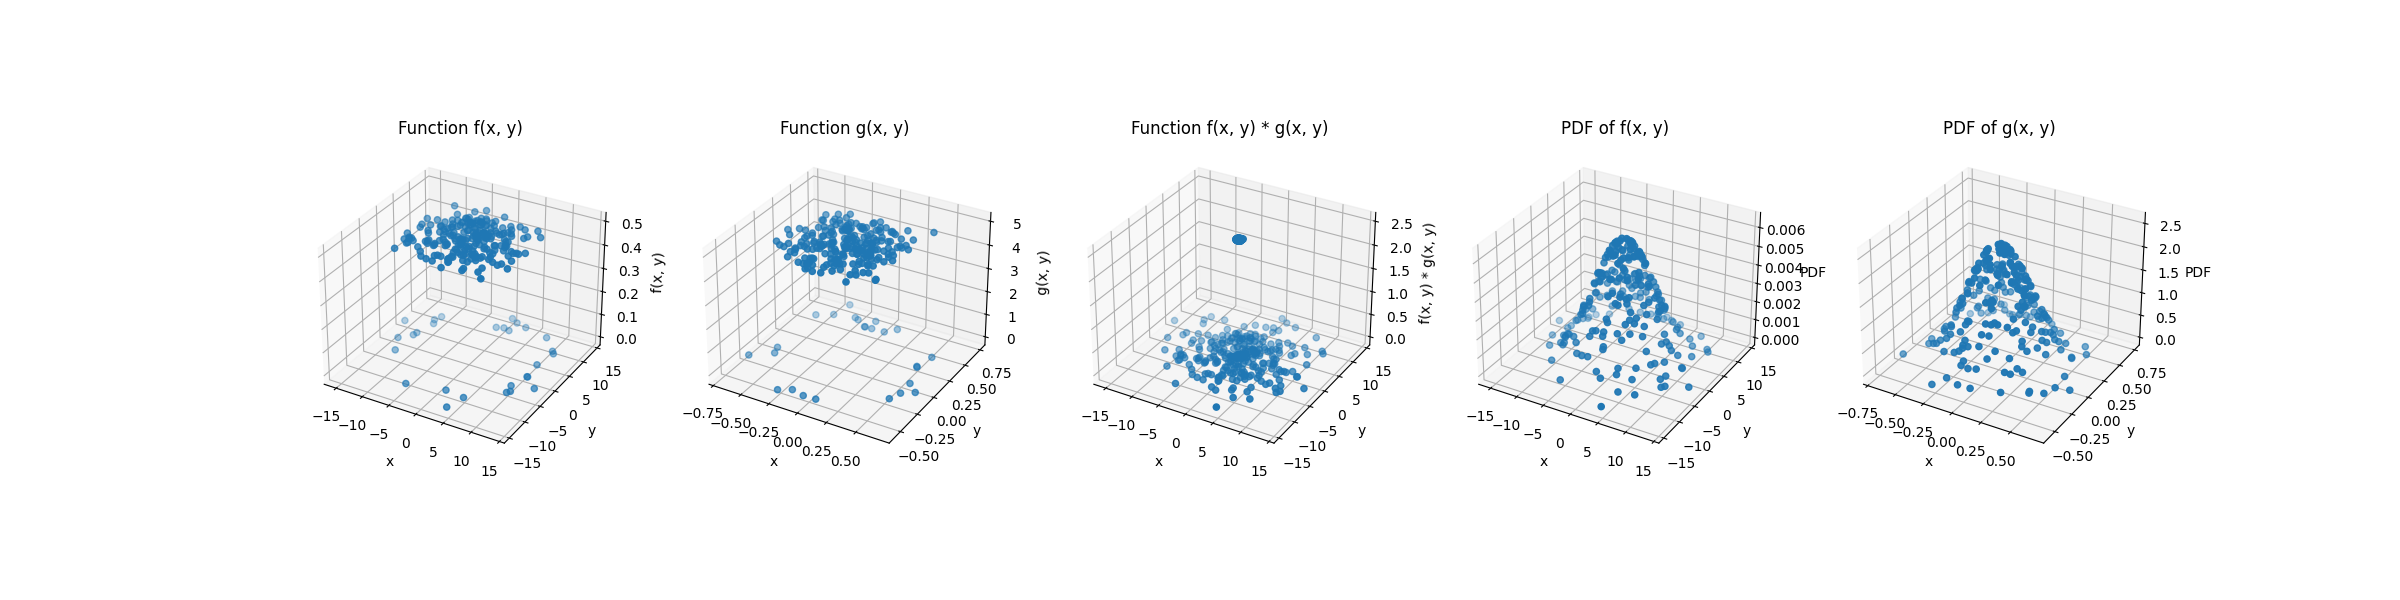
\includegraphics[width=1\textwidth]{balance_heuristic.png}
\caption{Funciones \( f(x) \) y \( g(x) \) en sus respectivos hipercubos, función \( f(x) \cdot g(x) \) y distribuciones de muestreo \( p_{i}(x) \) para cada rango \( [a_{i}, b_{i}] \).}
\label{fig:mis3}
\end{figure}

\subsubsection{Pruebas realizadas}

Sobre este caso de prueba se generó un análisis de las distintas heurísticas implementadas.
El análisis de este ejemplo se hizo de manera diferente a los anteriores y se corrieron todos los tests con los mismos hipercubos.
Entonces:
\begin{itemize}
\item Se hicieron 10 tests diferentes. Para cada test se utlizaron los mismos valores para \( a_{fi} \), \( b_{fi} \), \( c_f \), \( a_{gi} \), \( b_{gi} \) y \( c_g \).
      Los valores para \( a_{fi} \) y \( b_{fi} \) son -10 y 10 respectivamente. \( c_f \) es 0.5.
      Los valores para \( a_{gi} \) y \( b_{gi} \) son -0.5 y 0.5 respectivamente. \( c_g \) es 5.
\item La dimensionalidad de los tests es \( n + 1 \) donde \( n \) toma los siguientes valores: 2, 3, 4, 5, 6, 10, 12, 15, 18, 20.
\item Para cada test se corrió MIS con las siguientes heurísticas: balance, power, maximum, cutoff y sbert.
\item Para cada heurística se corrió MIS con 25, 50, 100, 500, 1000, 5000 y 50000 muestras.
\item Para cada heurística y cantidad de muestras se corrió MIS 100 veces y se calculó el promedio de las estimaciones,
      el promedio de la varianza de las estimaciones y el promedio de las desviaciones estándar de las estimaciones.
      A su vez, se calculó el promedio de los errores comparados el valor exacto de la integral y el promedio del tiempo de cómputo.
\end{itemize}

Luego, el análisis se hizo de la misma manera que en las pruebas anteriores.

\subsubsection{Resultados}

\begin{table}[H]
\centering
\label{table:heuristic_sample_analysis}
\small
\setlength{\tabcolsep}{3pt}
\renewcommand{\arraystretch}{1.2}
\begin{tabular}{|l|r|r|r|r|r|r|r|}
\hline
\textbf{\makecell{Heurística / \\ \# de muestras}} & \textbf{25} & \textbf{50} & \textbf{100} & \textbf{500} & \textbf{1000} & \textbf{5000} & \textbf{50000} \\ \hline
\multicolumn{8}{|c|}{\textbf{Promedio de Var}} \\ \hline
Balance & 83.88 & 5.48 & 10.06 & 16.93 & 4.61 & 25.98 & 78.95 \\ \hline
Power & 8.37 & 14.03 & 19.82 & 1.74 & 12.64 & 25.50 & 78.43 \\ \hline
Maximum & 159.54 & 60.44 & 41.34 & 11.77 & 18.73 & 5.72 & 4.50 \\ \hline
Cutoff & 42.11 & 43.85 & 8.61 & 16.80 & 4.83 & 25.96 & 3.60 \\ \hline
Sbert & 41.98 & 25.07 & 11.88 & 2.49 & 5.01 & 25.56 & 2.11 \\ \hline
\multicolumn{8}{|c|}{\textbf{Promedio de Err}} \\ \hline
Balance & 0.76 & 1.11 & 0.94 & 0.93 & 0.96 & 0.73 & 0.34 \\ \hline
Power & 1.02 & 1.00 & 0.78 & 1.04 & 0.77 & 0.76 & 0.37 \\ \hline
Maximum & -0.41 & -0.31 & -0.60 & -0.46 & -0.50 & -0.67 & -0.83 \\ \hline
Cutoff & 1.04 & 0.66 & 1.05 & 0.94 & 0.92 & 0.75 & 0.63 \\ \hline
Sbert & 0.93 & 0.93 & 0.94 & 0.97 & 0.90 & 0.74 & 0.76 \\ \hline
\multicolumn{8}{|c|}{\textbf{Promedio de DE}} \\ \hline
Balance & 1.24 & 0.78 & 0.81 & 0.59 & 0.47 & 0.54 & 0.72 \\ \hline
Power & 0.97 & 0.88 & 0.99 & 0.50 & 0.66 & 0.51 & 0.71 \\ \hline
Maximum & 1.89 & 1.57 & 1.64 & 1.02 & 0.88 & 0.71 & 0.50 \\ \hline
Cutoff & 0.97 & 1.19 & 0.72 & 0.59 & 0.51 & 0.52 & 0.42 \\ \hline
Sbert & 1.06 & 0.93 & 0.82 & 0.56 & 0.52 & 0.52 & 0.31 \\ \hline
\end{tabular}
\caption{Análisis de los resultados por heurística y cantidad de muestras}
\end{table}

\begin{table}[H]
\centering
\label{table:heuristic_test_analysis}
\resizebox{\textwidth}{!}{%
\begin{tabular}{|c|c|c|c|}
\hline
\textbf{Heurística/Test} & \textbf{Promedio de Var} & \textbf{Promedio de Err} & \textbf{Promedio de DE} \\ \hline
\multicolumn{4}{|c|}{\textbf{Test 1 (3 dimensiones)}} \\ \hline
Balance & 4.99 & -0.038 & 0.92 \\ \hline
Power & 7.62 & -0.215 & 1.11 \\ \hline
Maximum & 17.32 & -2.37 & 1.67 \\ \hline
Cutoff & 4.45 & 0.016 & 0.86 \\ \hline
Sbert & 6.67 & -0.106 & 0.96 \\ \hline
\multicolumn{4}{|c|}{\textbf{Test 2 (4 dimensiones)}} \\ \hline
Balance & 112.57 & -0.084 & 1.32 \\ \hline
Power & 41.46 & -0.107 & 1.35 \\ \hline
Maximum & 312.36 & -2.44 & 2.43 \\ \hline
Cutoff & 121.58 & -0.488 & 1.73 \\ \hline
Sbert & 96.73 & -0.375 & 1.59 \\ \hline
\multicolumn{4}{|c|}{\textbf{Test 3 (5 dimensiones)}} \\ \hline
Balance & 30.21 & 0.636 & 0.80 \\ \hline
Power & 18.34 & 0.700 & 0.74 \\ \hline
Maximum & 30.56 & -0.766 & 1.14 \\ \hline
Cutoff & 29.77 & 0.609 & 0.80 \\ \hline
Sbert & 7.62 & 0.833 & 0.60 \\ \hline
\multicolumn{4}{|c|}{\textbf{Test 4 (6 dimensiones)}} \\ \hline
Balance & 38.13 & 0.814 & 0.68 \\ \hline
Power & 37.52 & 0.820 & 0.68 \\ \hline
Maximum & 6.52 & -0.206 & 0.72 \\ \hline
Cutoff & 40.02 & 0.735 & 0.76 \\ \hline
Sbert & 37.37 & 0.852 & 0.64 \\ \hline
\multicolumn{4}{|c|}{\textbf{Test 5 (7 dimensiones)}} \\ \hline
Balance & 109.74 & 0.655 & 0.87 \\ \hline
Power & 109.28 & 0.686 & 0.85 \\ \hline
Maximum & 2.66 & -0.104 & 0.66 \\ \hline
Cutoff & 0.38 & 1.217 & 0.32 \\ \hline
Sbert & 0.57 & 1.226 & 0.31 \\ \hline
\end{tabular}%
}
\caption{Análisis de los resultados por heurística en los tests 1-5}
\end{table}

\begin{table}[H]
\centering
\label{table:heuristic_test_analysis}
\resizebox{\textwidth}{!}{%
\begin{tabular}{|c|c|c|c|}
\hline
\textbf{Heurística/Test} & \textbf{Promedio de Var} & \textbf{Promedio de Err} & \textbf{Promedio de DE} \\ \hline
\multicolumn{4}{|c|}{\textbf{Test 6 (11 dimensiones)}} \\ \hline
Balance & 1.68 & 1.265 & 0.41 \\ \hline
Power & 2.27 & 1.190 & 0.46 \\ \hline
Maximum & 2.10 & 0.095 & 0.77 \\ \hline
Cutoff & 1.19 & 1.234 & 0.43 \\ \hline
Sbert & 0.68 & 1.306 & 0.38 \\ \hline
\multicolumn{4}{|c|}{\textbf{Test 7 (13 dimensiones)}} \\ \hline
Balance & 0.88 & 1.294 & 0.44 \\ \hline
Power & 2.60 & 1.243 & 0.48 \\ \hline
Maximum & 3.59 & 0.072 & 0.86 \\ \hline
Cutoff & 1.18 & 1.256 & 0.48 \\ \hline
Sbert & 0.73 & 1.292 & 0.43 \\ \hline
\multicolumn{4}{|c|}{\textbf{Test 8 (16 dimensiones)}} \\ \hline
Balance & 2.77 & 1.259 & 0.54 \\ \hline
Power & 2.11 & 1.265 & 0.55 \\ \hline
Maximum & 11.72 & -0.016 & 1.13 \\ \hline
Cutoff & 5.39 & 1.199 & 0.61 \\ \hline
Sbert & 3.23 & 1.256 & 0.57 \\ \hline
\multicolumn{4}{|c|}{\textbf{Test 9 (19 dimensiones)}} \\ \hline
Balance & 4.73 & 1.264 & 0.63 \\ \hline
Power & 2.87 & 1.302 & 0.60 \\ \hline
Maximum & 5.19 & 0.405 & 0.88 \\ \hline
Cutoff & 0.72 & 1.414 & 0.47 \\ \hline
Sbert & 5.63 & 1.278 & 0.60 \\ \hline
\multicolumn{4}{|c|}{\textbf{Test 10 (21 dimensiones)}} \\ \hline
Balance & 17.01 & 1.180 & 0.75 \\ \hline
Power & 5.24 & 1.314 & 0.64 \\ \hline
Maximum & 39.47 & -0.077 & 1.45 \\ \hline
Cutoff & 3.54 & 1.375 & 0.56 \\ \hline
Sbert & 3.79 & 1.265 & 0.67 \\ \hline
\end{tabular}%
}
\caption{Análisis de los resultados por heurística en los tests 6-10}
\end{table}

\begin{table}[H]
\centering
\label{table:heuristic_analysis}
\begin{tabular}{|c|c|c|c|}
\hline
\textbf{Heurística} & \textbf{Promedio de Var} & \textbf{Promedio de Err} & \textbf{Promedio de DE} \\ \hline
Balance & 32.27 & 0.825 & 0.736 \\ \hline
Power & 22.93 & 0.820 & 0.746 \\ \hline
Maximum & 43.15 & -0.541 & 1.172 \\ \hline
Cutoff & 20.82 & 0.857 & 0.704 \\ \hline
Sbert & 16.30 & 0.883 & 0.675 \\ \hline
\end{tabular}
\caption{Análisis de los resultados por heurística}
\end{table}


\subsubsection{Análisis}

\paragraph{Varianza de las Estimaciones}
En términos de varianza, la heurística 'Balance' muestra un rendimiento consistentemente bueno, con una disminución notable en la varianza al aumentar el tamaño de la muestra. 'Sbert' también se destaca por tener varianzas bajas, lo que indica una mayor estabilidad en sus estimaciones. Por el contrario, 'Maximum' muestra la mayor variabilidad, lo que sugiere una menor fiabilidad y estabilidad en sus resultados.


\paragraph{Error de las Estimaciones}
Respecto a los errores, 'Balance' y 'Sbert' mantienen errores bajos y consistentes a través de los diferentes tamaños de muestra, lo que implica una mayor precisión en sus estimaciones. En cambio, 'Maximum' se inclina hacia errores negativos, indicando una tendencia a la subestimación. 'Cutoff' y 'Power' muestran más variabilidad en sus errores, lo que sugiere una precisión menos consistente.

\paragraph{Desviaciones Estándar de las Estimaciones}
Las desviaciones estándar más bajas se observan en las heurísticas 'Balance' y 'Sbert', lo que señala una mayor precisión y fiabilidad en sus estimaciones. 'Power', 'Maximum' y 'Cutoff' muestran desviaciones estándar más altas y variables, lo que refleja una consistencia y precisión menos fiables.

\paragraph{Dimensionalidad}
La dimensionalidad afecta significativamente el rendimiento de las heurísticas. En dimensiones más bajas, todas las heurísticas muestran un buen rendimiento. Sin embargo, en dimensiones más altas, 'Balance' y 'Sbert' logran mantener un control más efectivo sobre la varianza y el error, mientras que 'Maximum' y 'Cutoff' experimentan un aumento significativo en la varianza y el error.

\paragraph{Conclusiones}
En resumen, 'Balance' y 'Sbert' emergen como las heurísticas más robustas y consistentes en la Prueba 3, demostrando una buena precisión y estabilidad a lo largo de diferentes tamaños de muestra y en varias dimensiones. En contraste, 'Maximum' muestra una tendencia a la subestimación y es menos confiable, especialmente en dimensiones más altas. 'Power' y 'Cutoff' ofrecen un rendimiento intermedio, pero su precisión y consistencia son menos predecibles en comparación con 'Balance' y 'Sbert'.

\section{Conclusiones}

Las pruebas realizadas en este trabajo muestran que el MIS es una buena técnica para la estimación de distintas integrales.
Se probó en un espacio amplio de dimensiones y con distintas heurísticas en cada caso.

El caso 1, que es el más simple, mostró que el MIS es efectivo en dimensiones bajas y que la heurística 'Balance' es la más efectiva.
Este caso fue útil para entender cómo funciona el MIS y cómo se comporta en un caso simple.

El caso 2, que es un caso más complejo, mostró que el MIS es efectivo en dimensiones más altas y que la heurística 'Balance' mostró de nuevo ser la más efectiva.
Este caso fue útil para entender cómo se comporta el MIS en dimensiones más altas y cómo se comporta con distintas heurísticas en estas condiciones.

El caso 3, nos ayudó a entender cómo funciona el MIS en un producto de hipercubos y cómo se comporta en dimensiones más altas.
Sirvió para hacer un análisis en donde se multiplica una función de baja integral con una de alta integral y ver cómo el MIS se comporta en este caso.
De vuelta, la heurística 'Balance' mostró ser la más efectiva.

En resumen, el MIS es una técnica efectiva para la estimación de integrales en espacios de alta dimensión y la heurística 'Balance' es la más efectiva en la mayoría de los casos.
Se vio que la heurística presentada por Sbert también es efectiva en la mayoría de los casos y que se comporta de manera muy similar a 'Balance'.

Se pudo observar que las funciones utilizadas claramente no aportan el contexto necesario para que las heurísticas 'Power' 'Maximum' y 'Cutoff'.
Como explicado en las primeras secciones, estas heurísticas son efectivas en contextos muy particulares que no son reflejados en estos casos de prueba.

Para más información se puede ver el repositorio de GitHub en el que se encuentra el código utilizado para este trabajo: \url{https://github.com/santiagolmedo/multiple_importance_sampling}.
En él, se encuentran los códigos utilizados para las pruebas y los todos los resultados obtenidos.

\section{Bibliografía}

\end{document}

\[ (\int_{\Omega} \sum_{i=1}^{n} \frac{w_{i}^{2}(x) * f^{2}(x)}{n_{i} * p_{i}(x)} \,d\mu(x)) - (\sum_{i=1}^{n} \frac{1}{n_{i}} * \mu_{i}^{2}) \]

where

\[ \mu_{i} = \int_{\Omega} w_{i}(x) * f(x) \,d\mu(x)\]

$1 \times 10^{6}$